% ==============================================================================
% SECTION 01: CURATED DOMAIN DATASET & SPLIT INTEGRITY
% AZN-Vision: Assistive Azerbaijani Banknote Recognition System
% Cohort I 2026 - AI Academy - National Artificial Intelligence Center
% Group: M001 | Team: Qarabağ Zəfəri
% ==============================================================================

% ------------------------------------------------------------------------------
% Slide 1 (Page 2): Domain Data Acquisition & Multi-Annotator Protocol
% ------------------------------------------------------------------------------
\begin{frame}{Domain Data Acquisition \& Multi-Annotator Protocol}{Gold-Standard Ground Truth with Proven Inter-Annotator Agreement}
    \begin{columns}[c]
        \begin{column}{0.54\textwidth}
            \begin{techblock}{In-the-Wild Numismatic Capture}
                \footnotesize
                \begin{itemize}\setlength{\itemsep}{2pt}
                    \item \textbf{Scope:} 7 circulating AZN notes (1 to 200 AZN).
                    \item \textbf{Raw Ingestion:} 2,593 captures across 93 unconstrained scenes.
                    \item \textbf{Data Hygiene:} 71 frames pruned (52 duplicates, 19 empty labels).
                    \item \textbf{Production Benchmark:} \textbf{2,522 active unique notes}.
                \end{itemize}
            \end{techblock}
            
            \vspace{0.12cm}
            \begin{alertblockcustom}{Multi-Annotator Calibration Protocol}
                \footnotesize
                \begin{itemize}\setlength{\itemsep}{2pt}
                    \item \textbf{Calibration Protocol:} 5 annotators on 150 benchmark images.
                    \item \textbf{Spatial IoU Agreement:} \textbf{93.4\%} ($\pm 0.028$, median: 94.8\%).
                    \item \textbf{Label Concordance:} \textbf{98.8\%} (Fleiss' $\kappa = 0.962$).
                \end{itemize}
            \end{alertblockcustom}
        \end{column}
        
        \begin{column}{0.44\textwidth}
            \begin{card}{Dataset Breakdown (2522 Clean Notes)}
                \centering
                \scriptsize
                \renewcommand{\arraystretch}{1.05}
                \begin{tabular}{l l r}
                    \toprule
                    \textbf{Denom} & \textbf{Numismatic Motif} & \textbf{Count} \\
                    \midrule
                    \textbf{001 AZN} & Tar \& Folk Culture & 439 \\
                    \textbf{005 AZN} & Literature \& Poetry & 297 \\
                    \textbf{010 AZN} & Old City Architecture & 493 \\
                    \textbf{020 AZN} & Military \& Karabakh & 314 \\
                    \textbf{050 AZN} & Education \& Youth & 321 \\
                    \textbf{100 AZN} & Modern Infrastructure & 377 \\
                    \textbf{200 AZN} & Modernist Architecture & 281 \\
                    \bottomrule
                \end{tabular}
            \end{card}
            
            \vspace{0.12cm}
            \kpitech{93.4\% Mean IoU}{5-Member Blinded Agreement Calibration}{Fleiss' $\kappa = 0.962$ verifies robust mutual ground truth}
        \end{column}
    \end{columns}
\end{frame}

% ------------------------------------------------------------------------------
% Slide 2 (Page 3): In-the-Wild Dataset Visual Showcase (Batch Sample Grid)
% ------------------------------------------------------------------------------
\begin{frame}{Authentic Numismatic Spectrum}{Real-World Capture Diversity Across All Circulating Denominations}
    \centering
    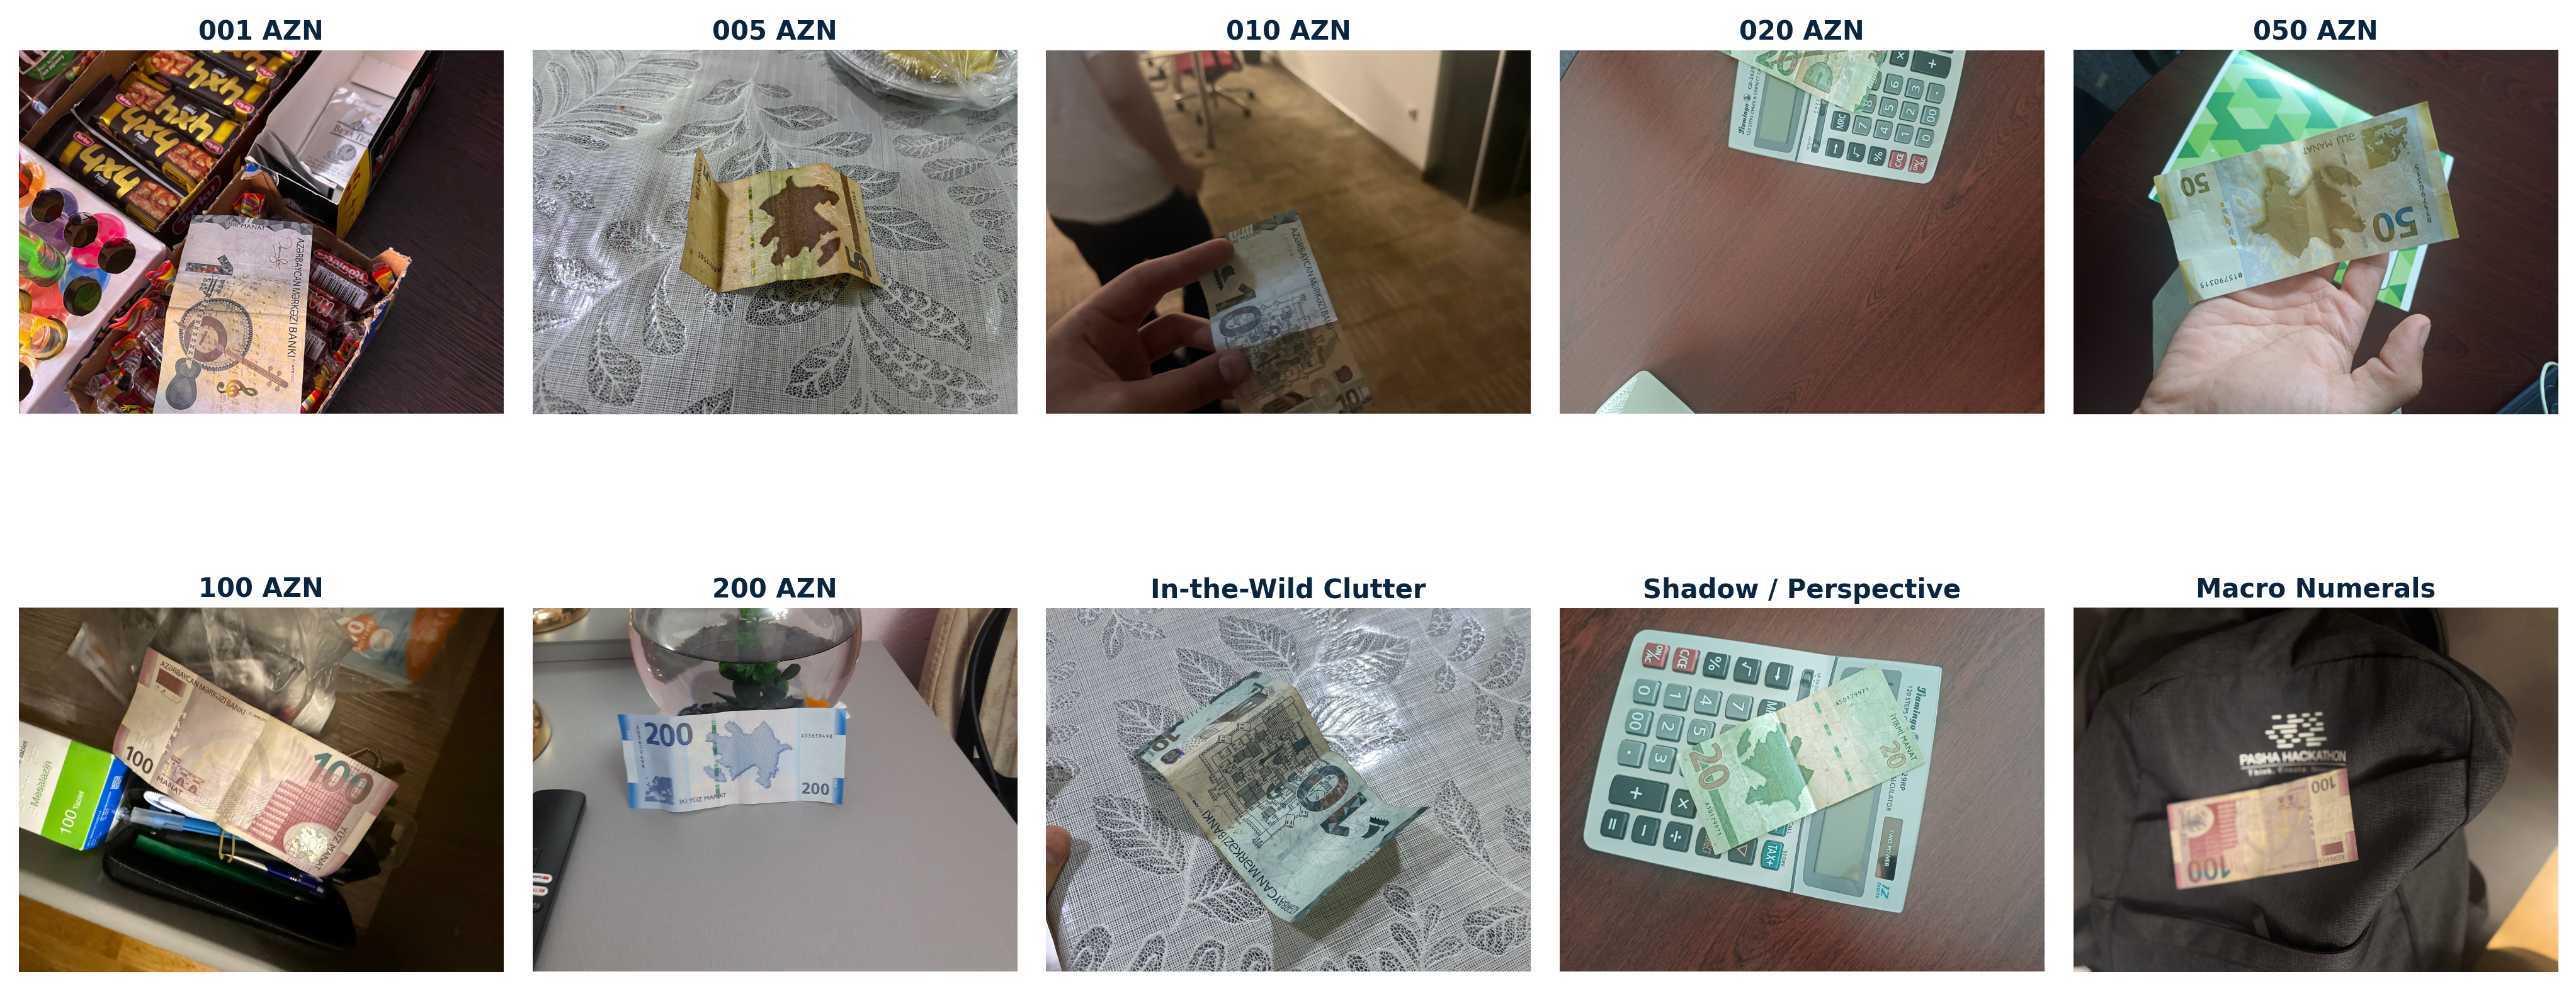
\includegraphics[width=0.96\textwidth,height=0.66\textheight,keepaspectratio]{../reports/figures/eda/dataset_sample_batch_grid.png}
    
    \vspace{0.12cm}
    \begin{columns}[T]
        \begin{column}{0.32\textwidth}
            \centering \scriptsize \textbf{Numismatic Spectrum}\\
            \tiny 7 distinct nominal color palettes \& micro-engravings.
        \end{column}
        \begin{column}{0.32\textwidth}
            \centering \scriptsize \textbf{Physical Stress Factors}\\
            \tiny Severe creases, crumples, heavy folds, and finger grips.
        \end{column}
        \begin{column}{0.32\textwidth}
            \centering \scriptsize \textbf{Unconstrained Clutter}\\
            \tiny Varied tabletops, harsh specular glare, and deep shadows.
        \end{column}
    \end{columns}
\end{frame}

% ------------------------------------------------------------------------------
% Slide 3 (Page 4): Perceptual Deduplication Pipeline (pHash & Laplacian)
% ------------------------------------------------------------------------------
\begin{frame}{Perceptual Deduplication \& Sharpness Hygiene}{Eliminating Burst-Shot Redundancy via DCT pHash and Laplacian Variance}
    \begin{columns}[c]
        \begin{column}{0.48\textwidth}
            \centering
            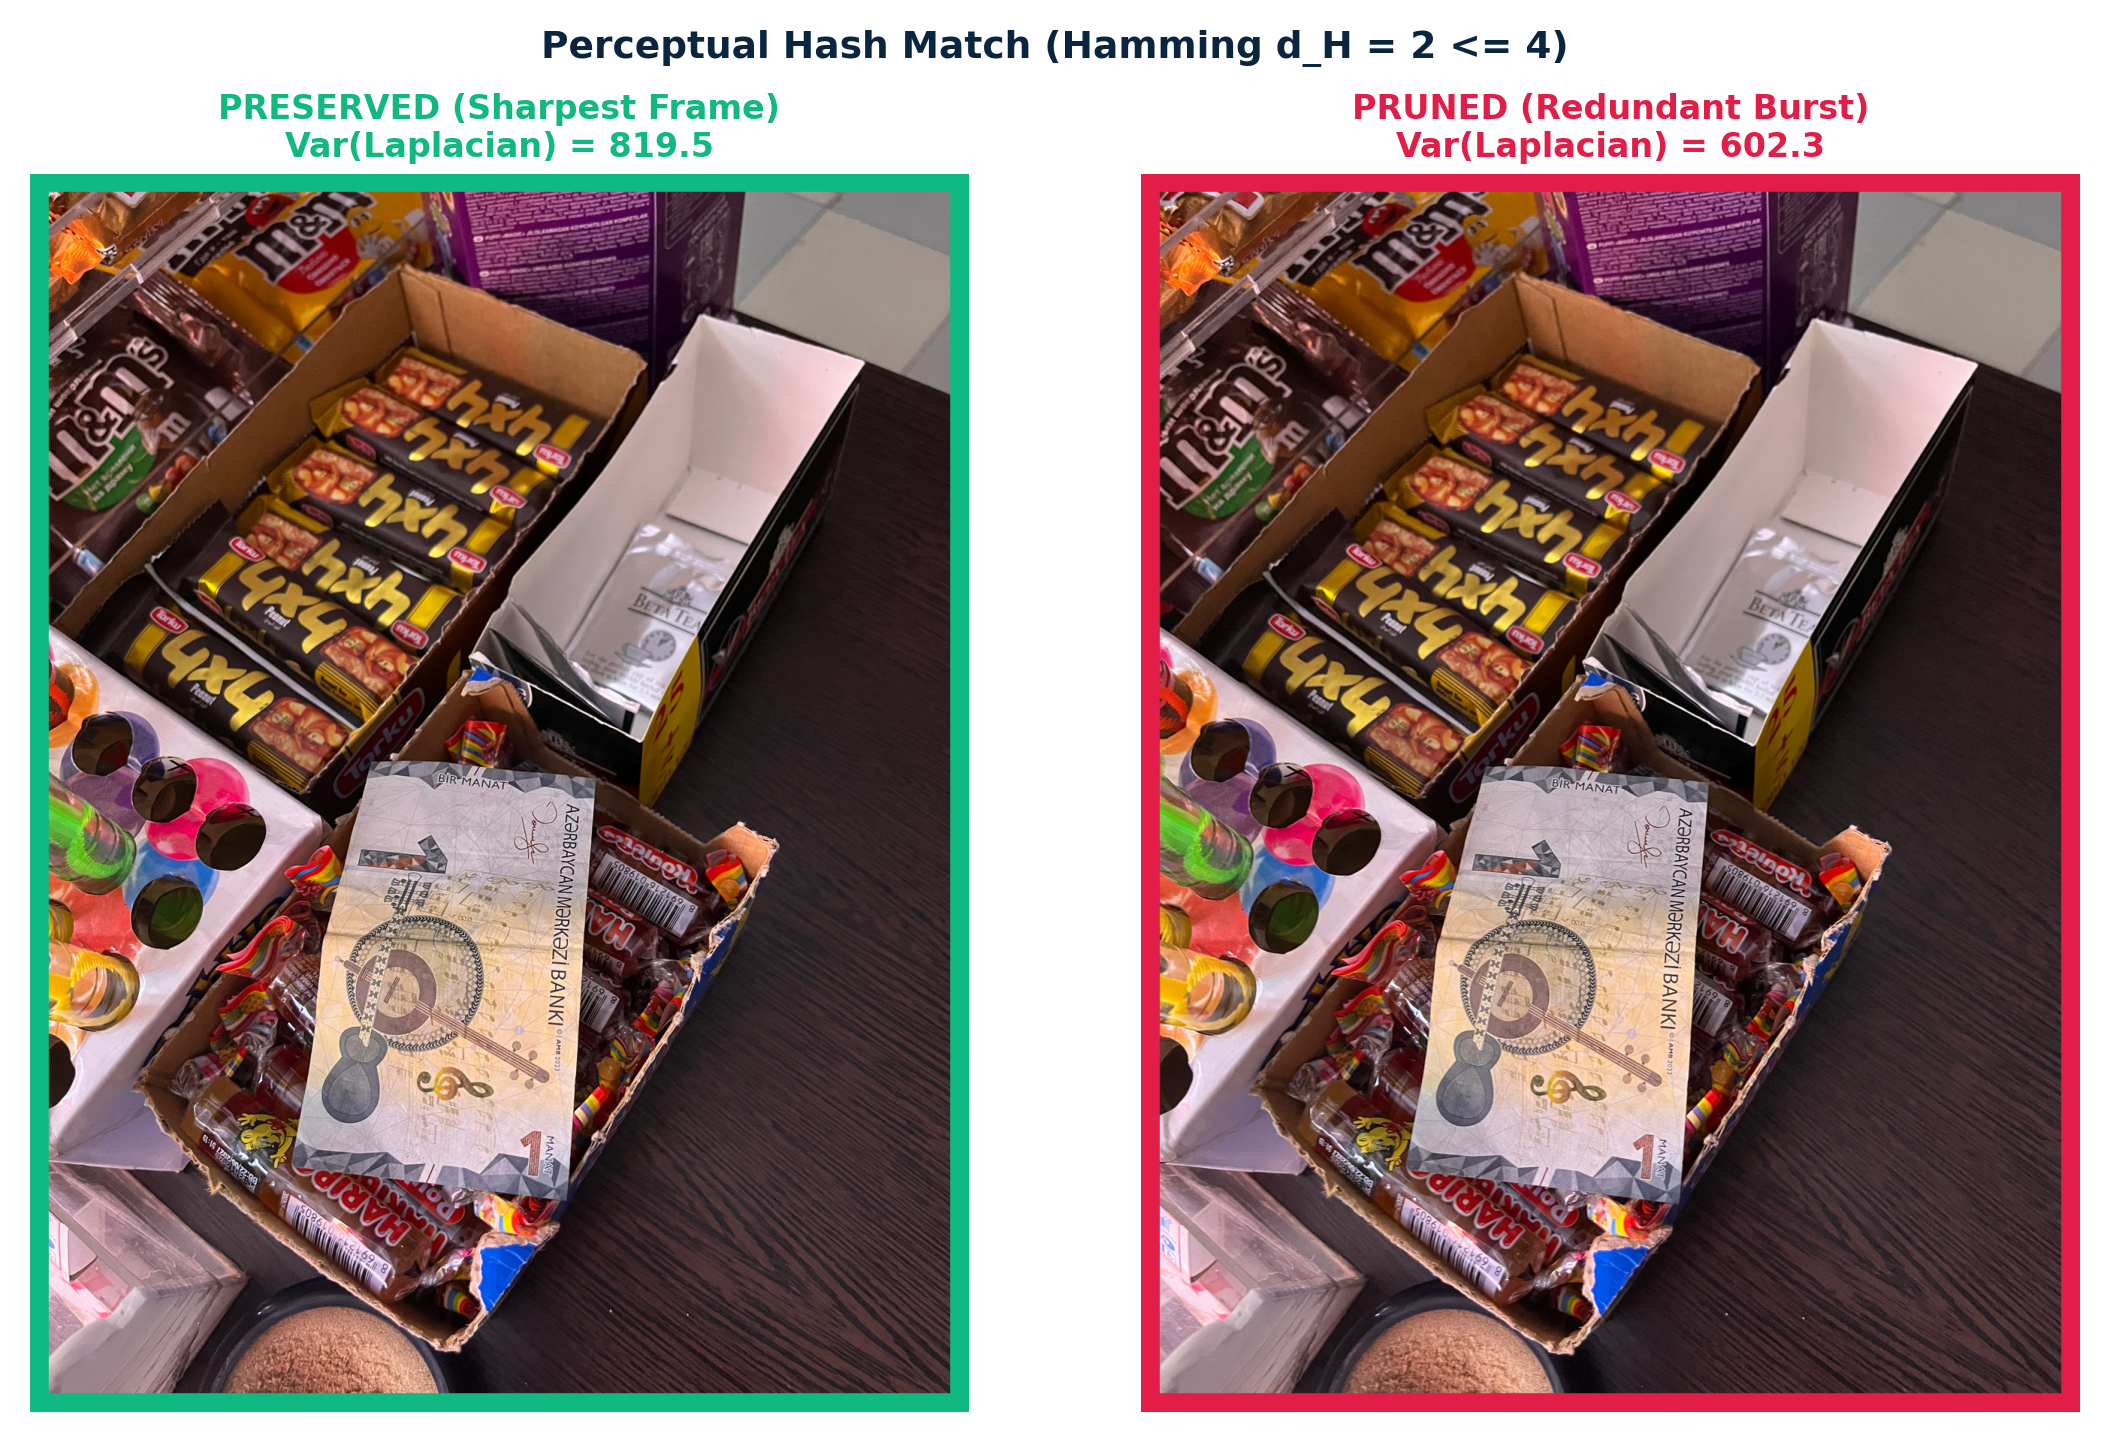
\includegraphics[width=\textwidth,height=0.70\textheight,keepaspectratio]{../reports/figures/eda/near_duplicate_pair_example.png}
        \end{column}
        
        \begin{column}{0.50\textwidth}
            \begin{techblock}{Dual-Stage Quality Gate (\texttt{deduplicate.py})}
                \scriptsize
                \begin{itemize}\setlength{\itemsep}{1.5pt}
                    \item \textbf{Raw Ingestion Pool:} 2,593 uncurated mobile frames.
                    \item \textbf{Exact SHA-256:} 3 bitwise identical duplicate frames pruned.
                    \item \textbf{DCT pHash ($d_H \le 4$):} 50 redundant clusters (49 burst frames pruned).
                    \item \textbf{Defective Annotations:} 19 unannotated/empty frames quarantined.
                    \item \textbf{Verified Clean Set:} \textbf{2,522 active unique notes} for modeling.
                \end{itemize}
            \end{techblock}
            
            \vspace{0.12cm}
            \begin{alertblockcustom}{Laplacian Sharpness Competition}
                \scriptsize
                \begin{itemize}\setlength{\itemsep}{1.5pt}
                    \item \textbf{Mathematical Operator:} $\text{Score}(I) = \mathrm{Var}(\nabla^2 I)$ over luminance.
                    \item \textbf{Preserved Canonical:} Frame with superior gradient energy ($819.5$).
                    \item \textbf{Quarantined Duplicates:} 49 motion-blurred copies ($602.3$), eliminating camera-shake memorization.
                \end{itemize}
            \end{alertblockcustom}
        \end{column}
    \end{columns}
\end{frame}

% ------------------------------------------------------------------------------
% Slide 4 (Page 5): Comprehensive EDA — Spatial Geometry & Boundary Distribution
% ------------------------------------------------------------------------------
\begin{frame}{Exploratory Data Analysis: Spatial Geometry}{Rigorous Profiling of Scale Variations, Aspect Ratios, and Boundary Proximity}
    \begin{columns}[c]
        \begin{column}{0.54\textwidth}
            \centering
            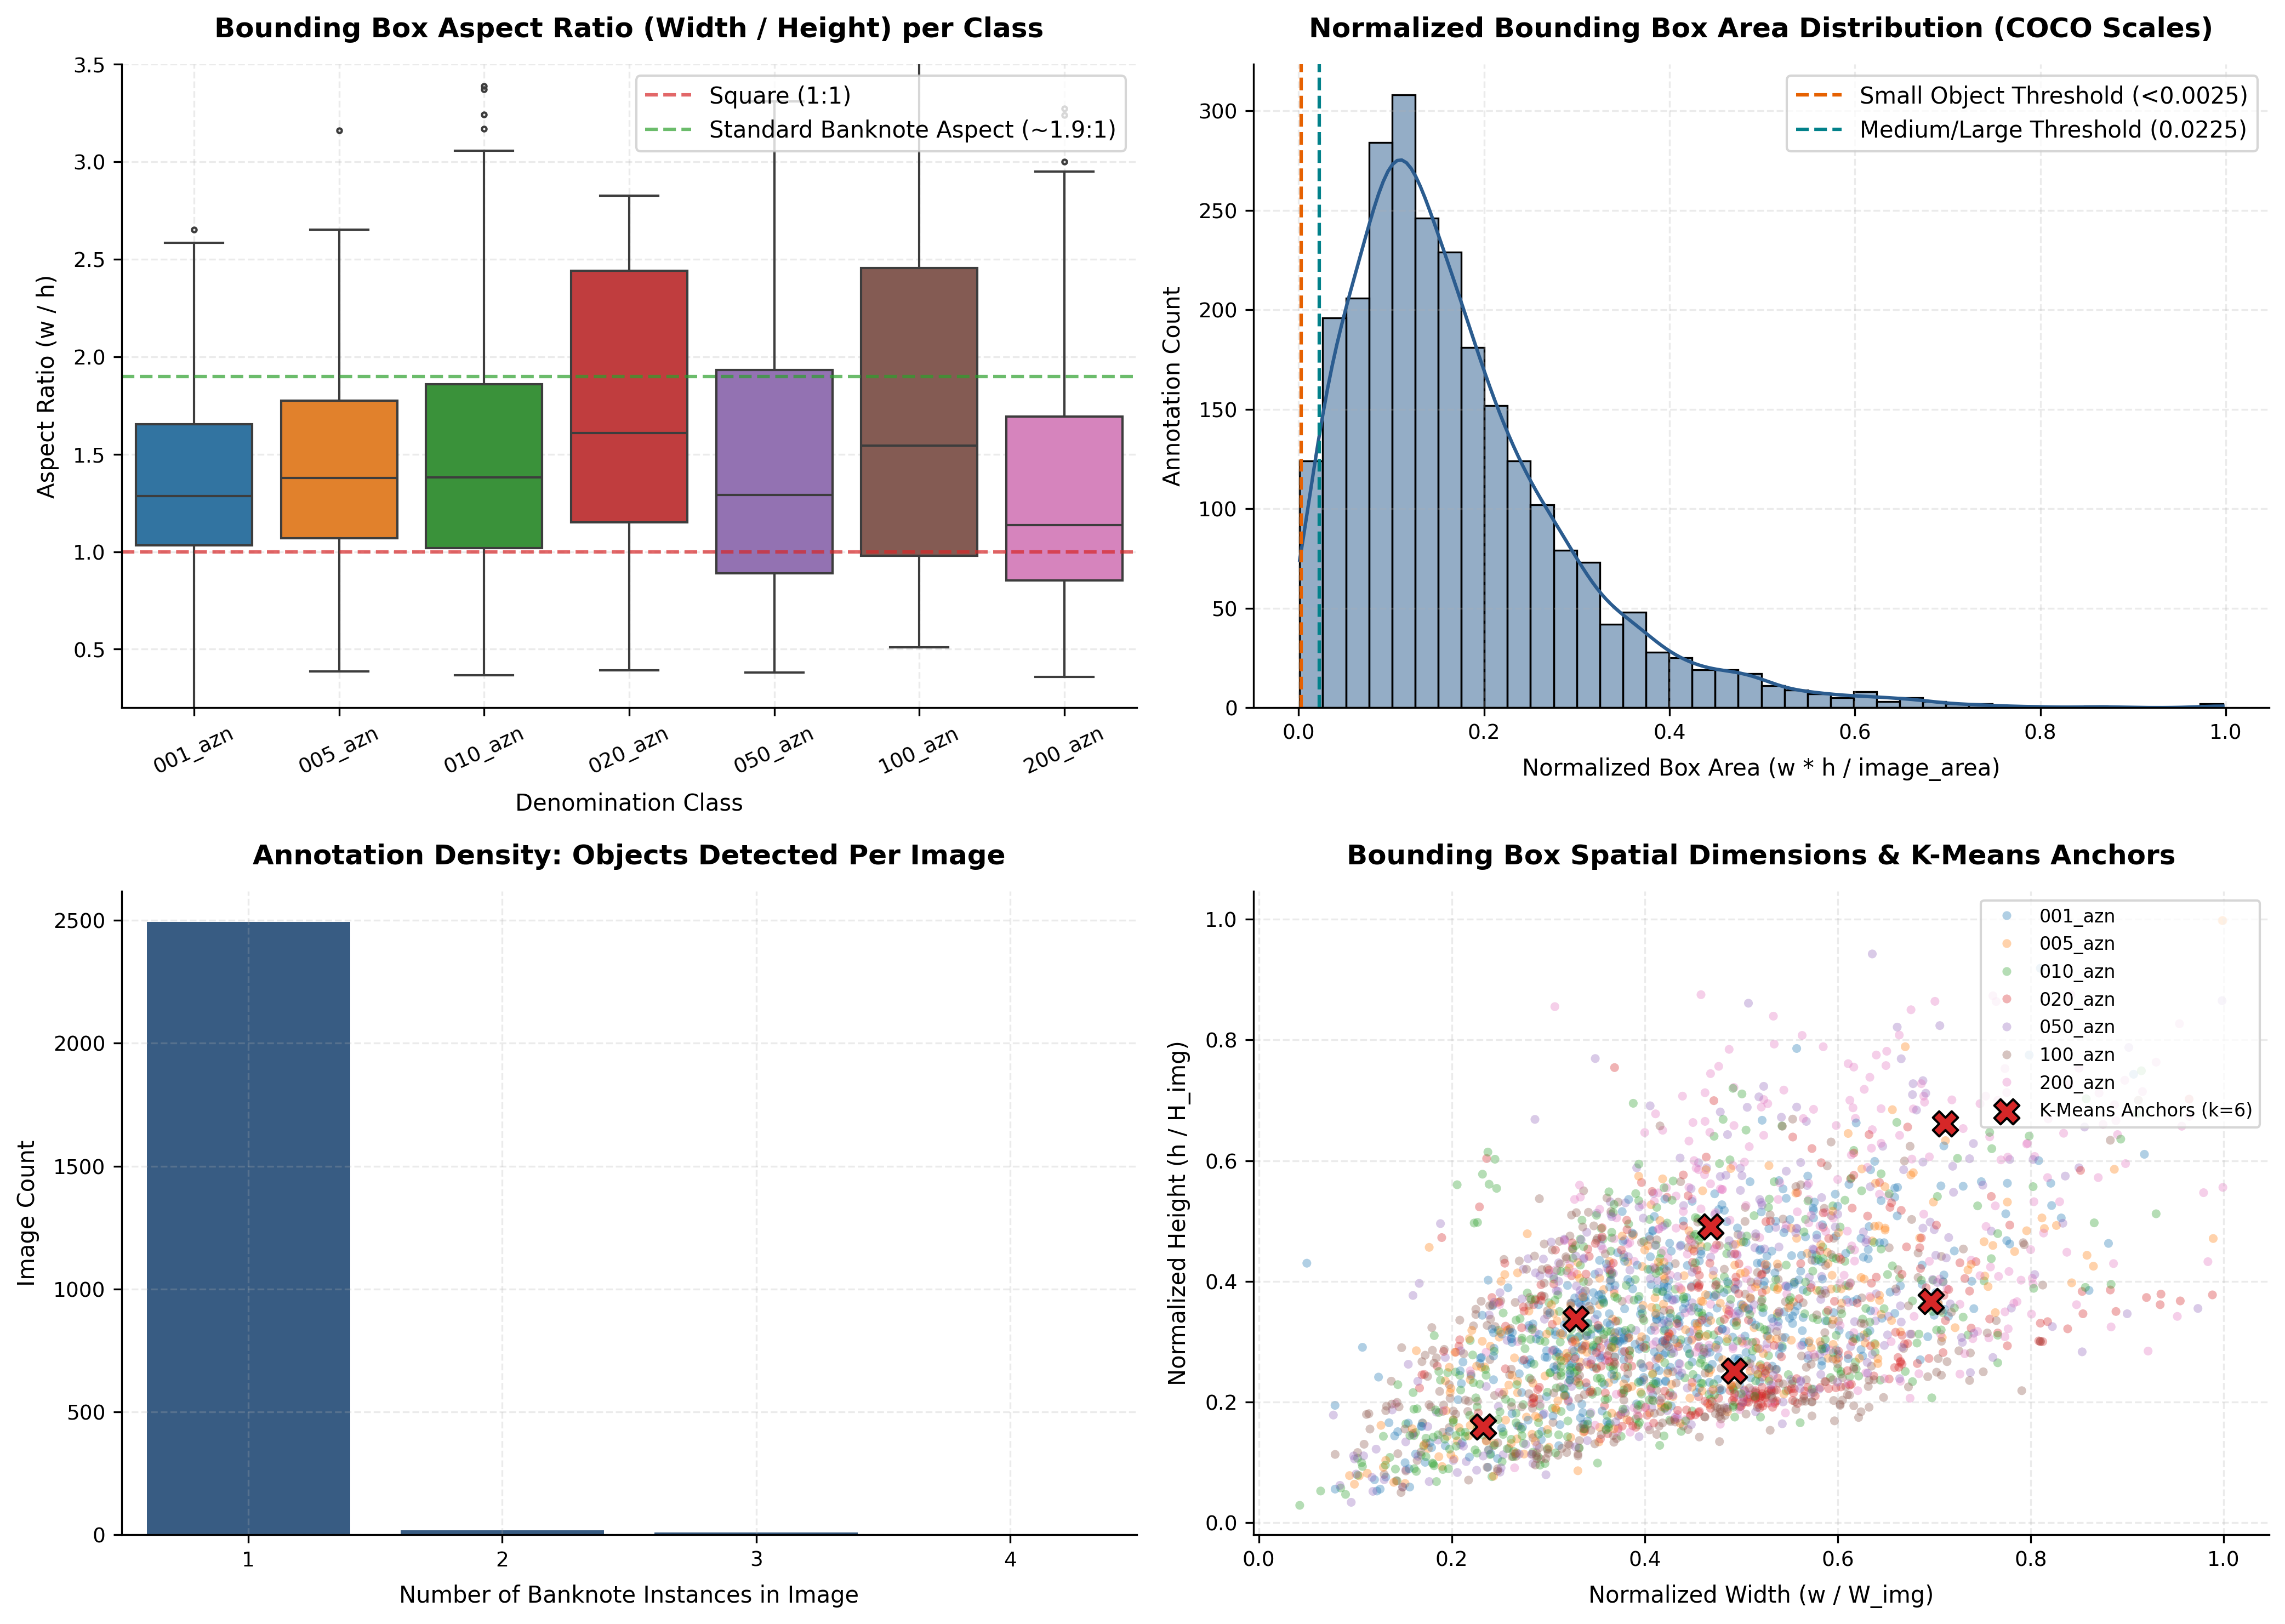
\includegraphics[width=\textwidth,height=0.74\textheight,keepaspectratio]{../reports/figures/eda/eda_spatial_geometry.png}
        \end{column}
        
        \begin{column}{0.44\textwidth}
            \begin{techblock}{Spatial Scale Dynamics}
                \scriptsize
                \begin{itemize}\setlength{\itemsep}{2pt}
                    \item \textbf{Multi-Scale Span:} $<5\%$ (distant) to $>80\%$ (macro).
                    \item \textbf{Aspect Ratio Spread:} Range $1.0\times\text{--}3.2\times$ (nominal: $1.9:1$).
                    \item \textbf{Boundary Proximity:} Edge-touching truncations.
                \end{itemize}
            \end{techblock}
            
            \vspace{0.12cm}
            \begin{card}{Engineering Takeaways}
                \scriptsize
                \begin{itemize}\setlength{\itemsep}{2.5pt}
                    \item \textbf{Anchor Dimensioning:} Bimodal scale demands 3-scale FPN with high-aspect anchor priors.
                    \item \textbf{Augmentation Rationale:} Rotation ($\pm 15^\circ$) + Mosaic prevent false boundary edge clipping.
                    \item \textbf{Edge Crop Policy:} Zero coordinate hallucination when banknote touches frame perimeter.
                \end{itemize}
            \end{card}
        \end{column}
    \end{columns}
\end{frame}

% ------------------------------------------------------------------------------
% Slide 5 (Page 6): Exploratory Data Analysis — Photometric & Sharpness Invariance
% ------------------------------------------------------------------------------
\begin{frame}{Exploratory Data Analysis: Photometric Invariance}{Empirical Luminance Spread, Color Channel Distributions, and Blur Profiles}
    \begin{columns}[c]
        \begin{column}{0.54\textwidth}
            \centering
            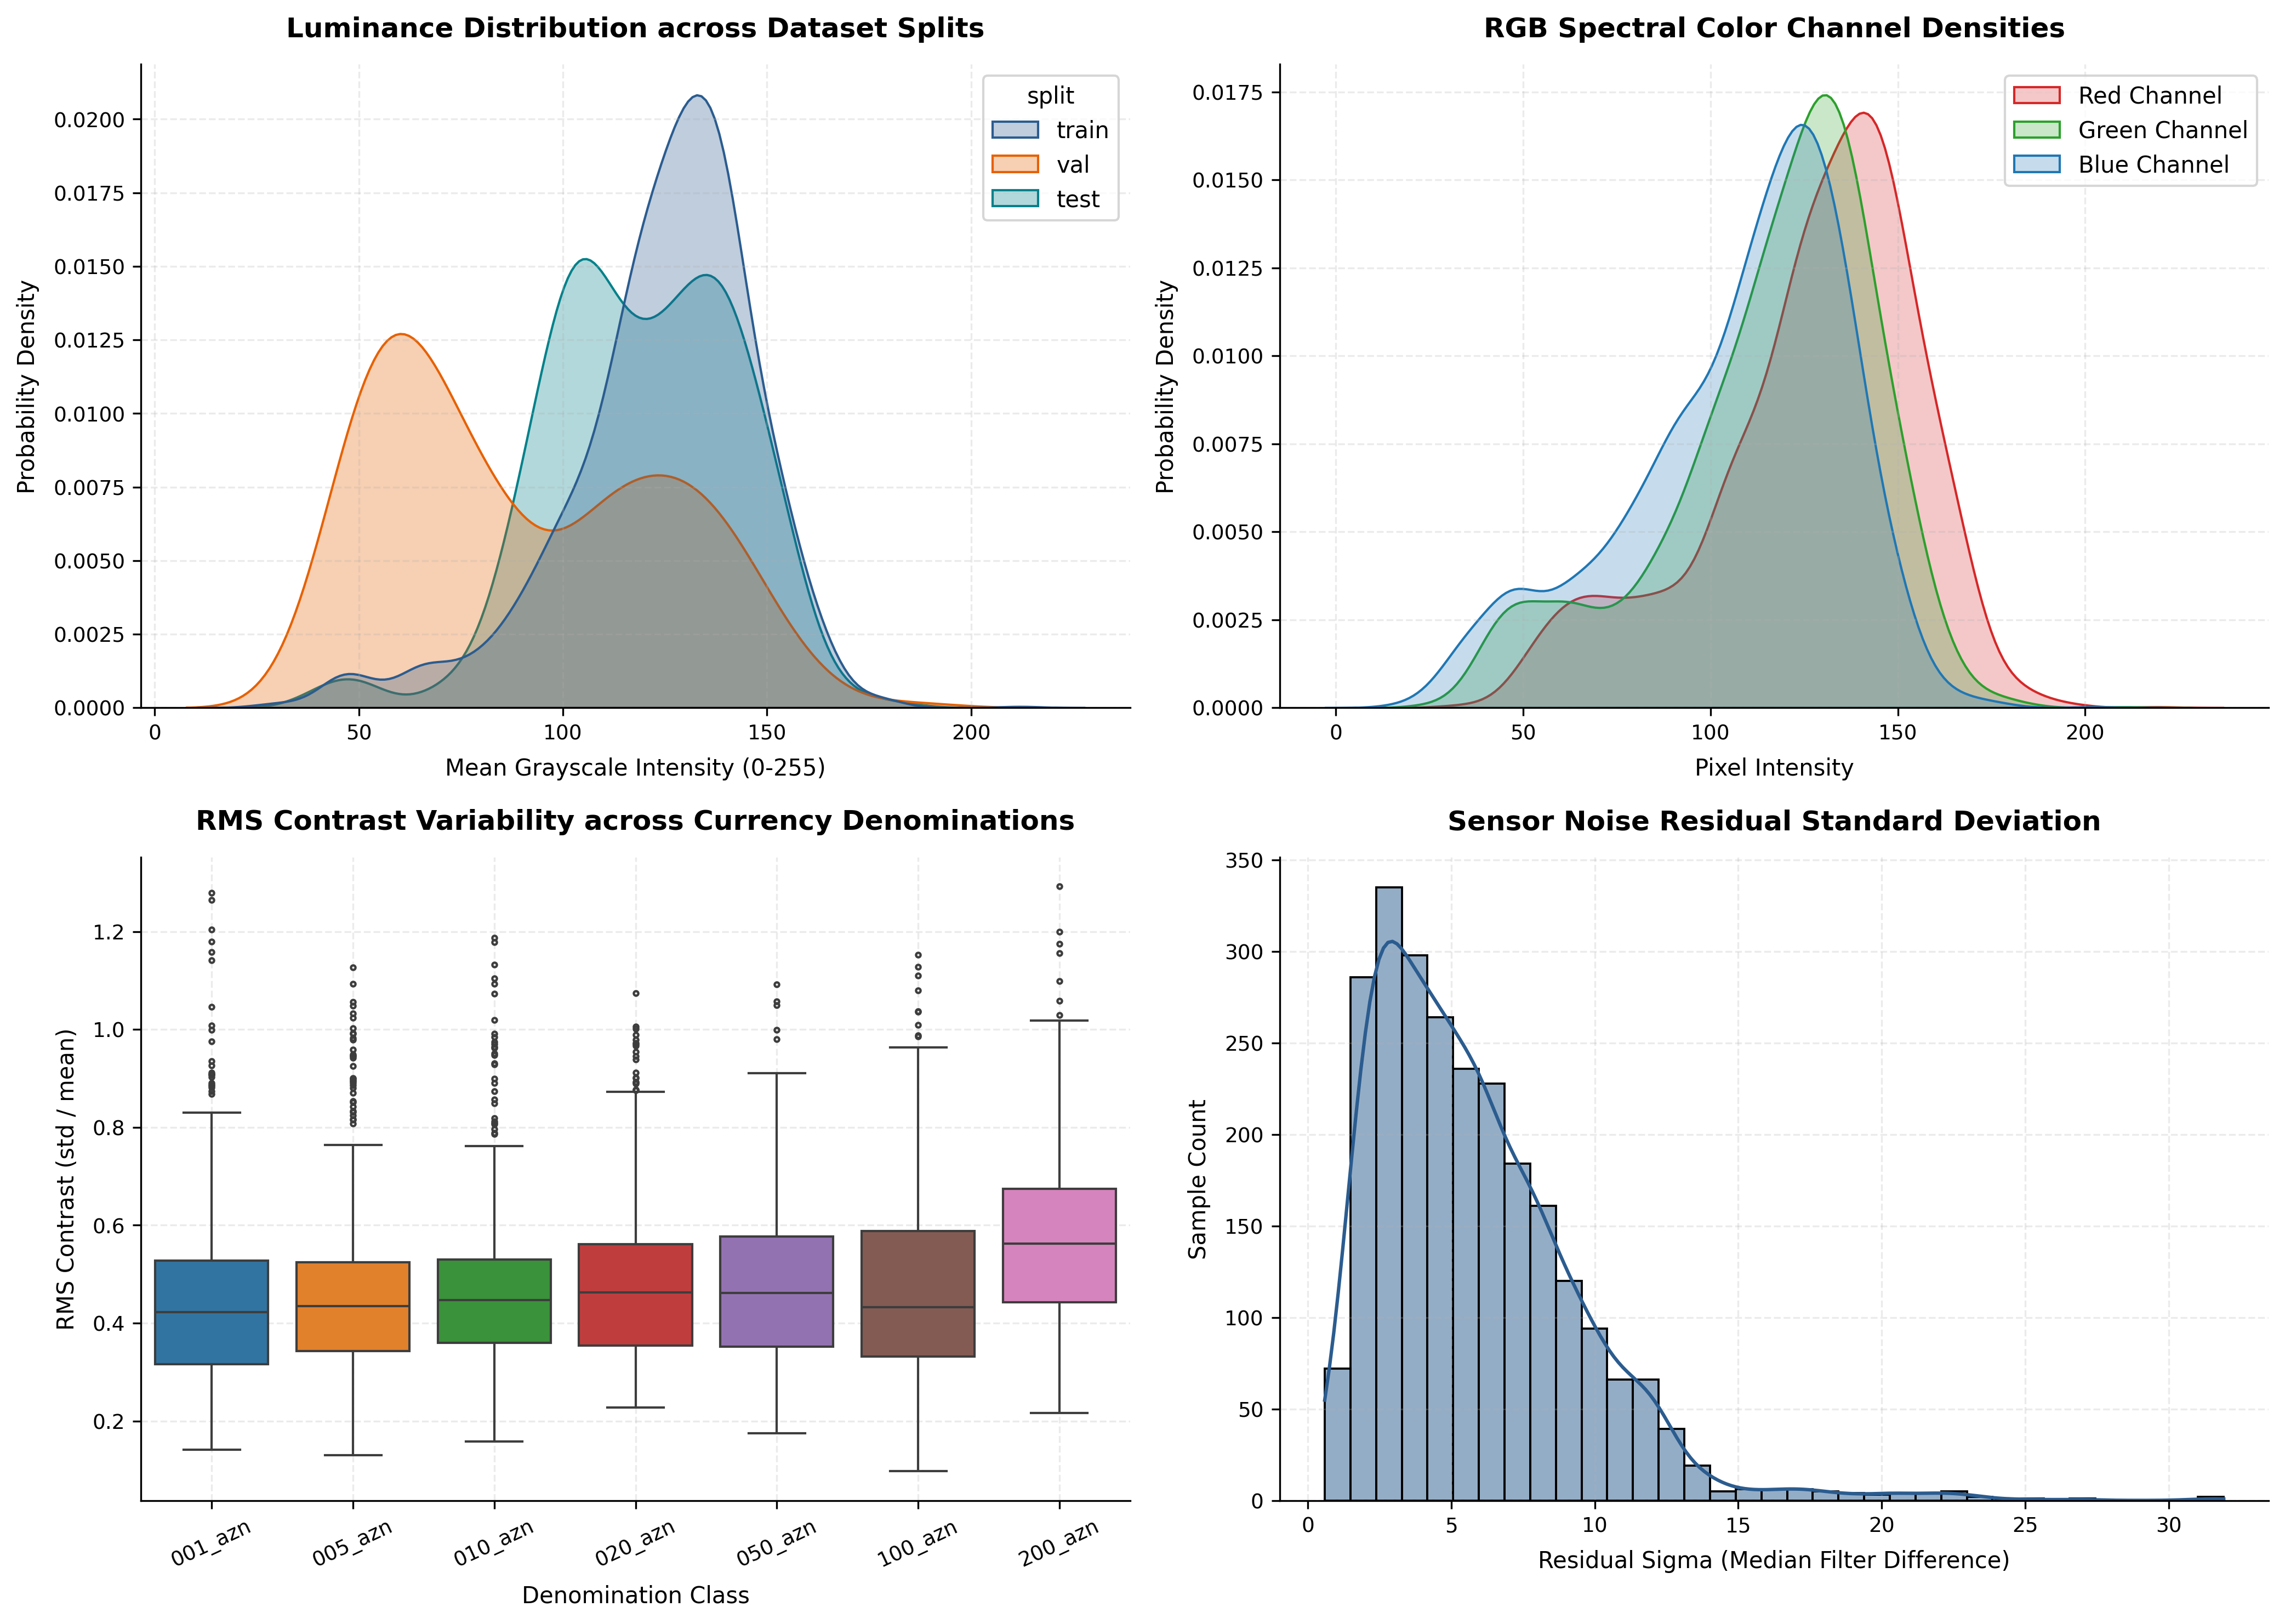
\includegraphics[width=\textwidth,height=0.74\textheight,keepaspectratio]{../reports/figures/eda/eda_photometric_distributions.png}
        \end{column}
        
        \begin{column}{0.44\textwidth}
            \begin{techblock}{Photometric Dynamics}
                \scriptsize
                \begin{itemize}\setlength{\itemsep}{2pt}
                    \item \textbf{Dynamic Range:} Extreme shadows ($\mu < 45$) to glare ($\mu > 215$).
                    \item \textbf{Color Spread:} Inter-channel white balance deviations.
                    \item \textbf{Motion Residuals:} Laplacian tail confirms handheld jitter.
                \end{itemize}
            \end{techblock}
            
            \vspace{0.12cm}
            \begin{card}{Engineering Takeaways}
                \scriptsize
                \begin{itemize}\setlength{\itemsep}{2.5pt}
                    \item \textbf{Sensor Tuning:} OV2640 on ESP32 requires automatic exposure locking (AEC) for banknote capture.
                    \item \textbf{HSV Jitter Necessity:} Random hue ($\pm 0.015$) \& saturation ($\pm 0.7$) prevent color shortcut memorization.
                    \item \textbf{Contrast Normalization:} CLAHE-inspired augmentation arms essential for low-light stability.
                \end{itemize}
            \end{card}
        \end{column}
    \end{columns}
\end{frame}

% ------------------------------------------------------------------------------
% Slide 6 (Page 7): The Spatial Leakage Trap & DINOv2 ViT-L/14 Semantic Manifold
% ------------------------------------------------------------------------------
\begin{frame}{The Spatial Leakage Trap \& DINOv2 Foundation Latents}{Preventing Benchmark Overfitting Through Self-Supervised Vision Clustering}
    \begin{columns}[c]
        \begin{column}{0.48\textwidth}
            \begin{alertblockcustom}{The CV Leakage Trap in Wearable Vision}
                \scriptsize
                \begin{itemize}\setlength{\itemsep}{1.5pt}
                    \item \textbf{Flawed Random Splits:} Distributes same desk/lighting burst frames across Train and Test (Hard/Soft Leakage).
                    \item \textbf{Artificial Benchmark:} Delivers fabricated 99.9\% mAP that collapses catastrophically in real-world deployment.
                \end{itemize}
            \end{alertblockcustom}
            
            \vspace{0.10cm}
            \begin{techblock}{DINOv2 ViT-L/14 Foundation Latents}
                \scriptsize
                \begin{itemize}\setlength{\itemsep}{1.5pt}
                    \item \textbf{Foundation Encoder:} Self-supervised ViT-L/14 frozen backbone.
                    \item \textbf{1024-dim Latent Space:} High-capacity semantic embeddings capturing scene environments without supervision.
                    \item \textbf{Meta-Scene Discovery:} Cosine affinity graph groups notes into \textbf{93 physically disjoint clusters}.
                    \item \textbf{Generalization Proof:} Validates zero room, tabletop, or lighting leakage across splits.
                \end{itemize}
            \end{techblock}
        \end{column}
        
        \begin{column}{0.50\textwidth}
            \centering
            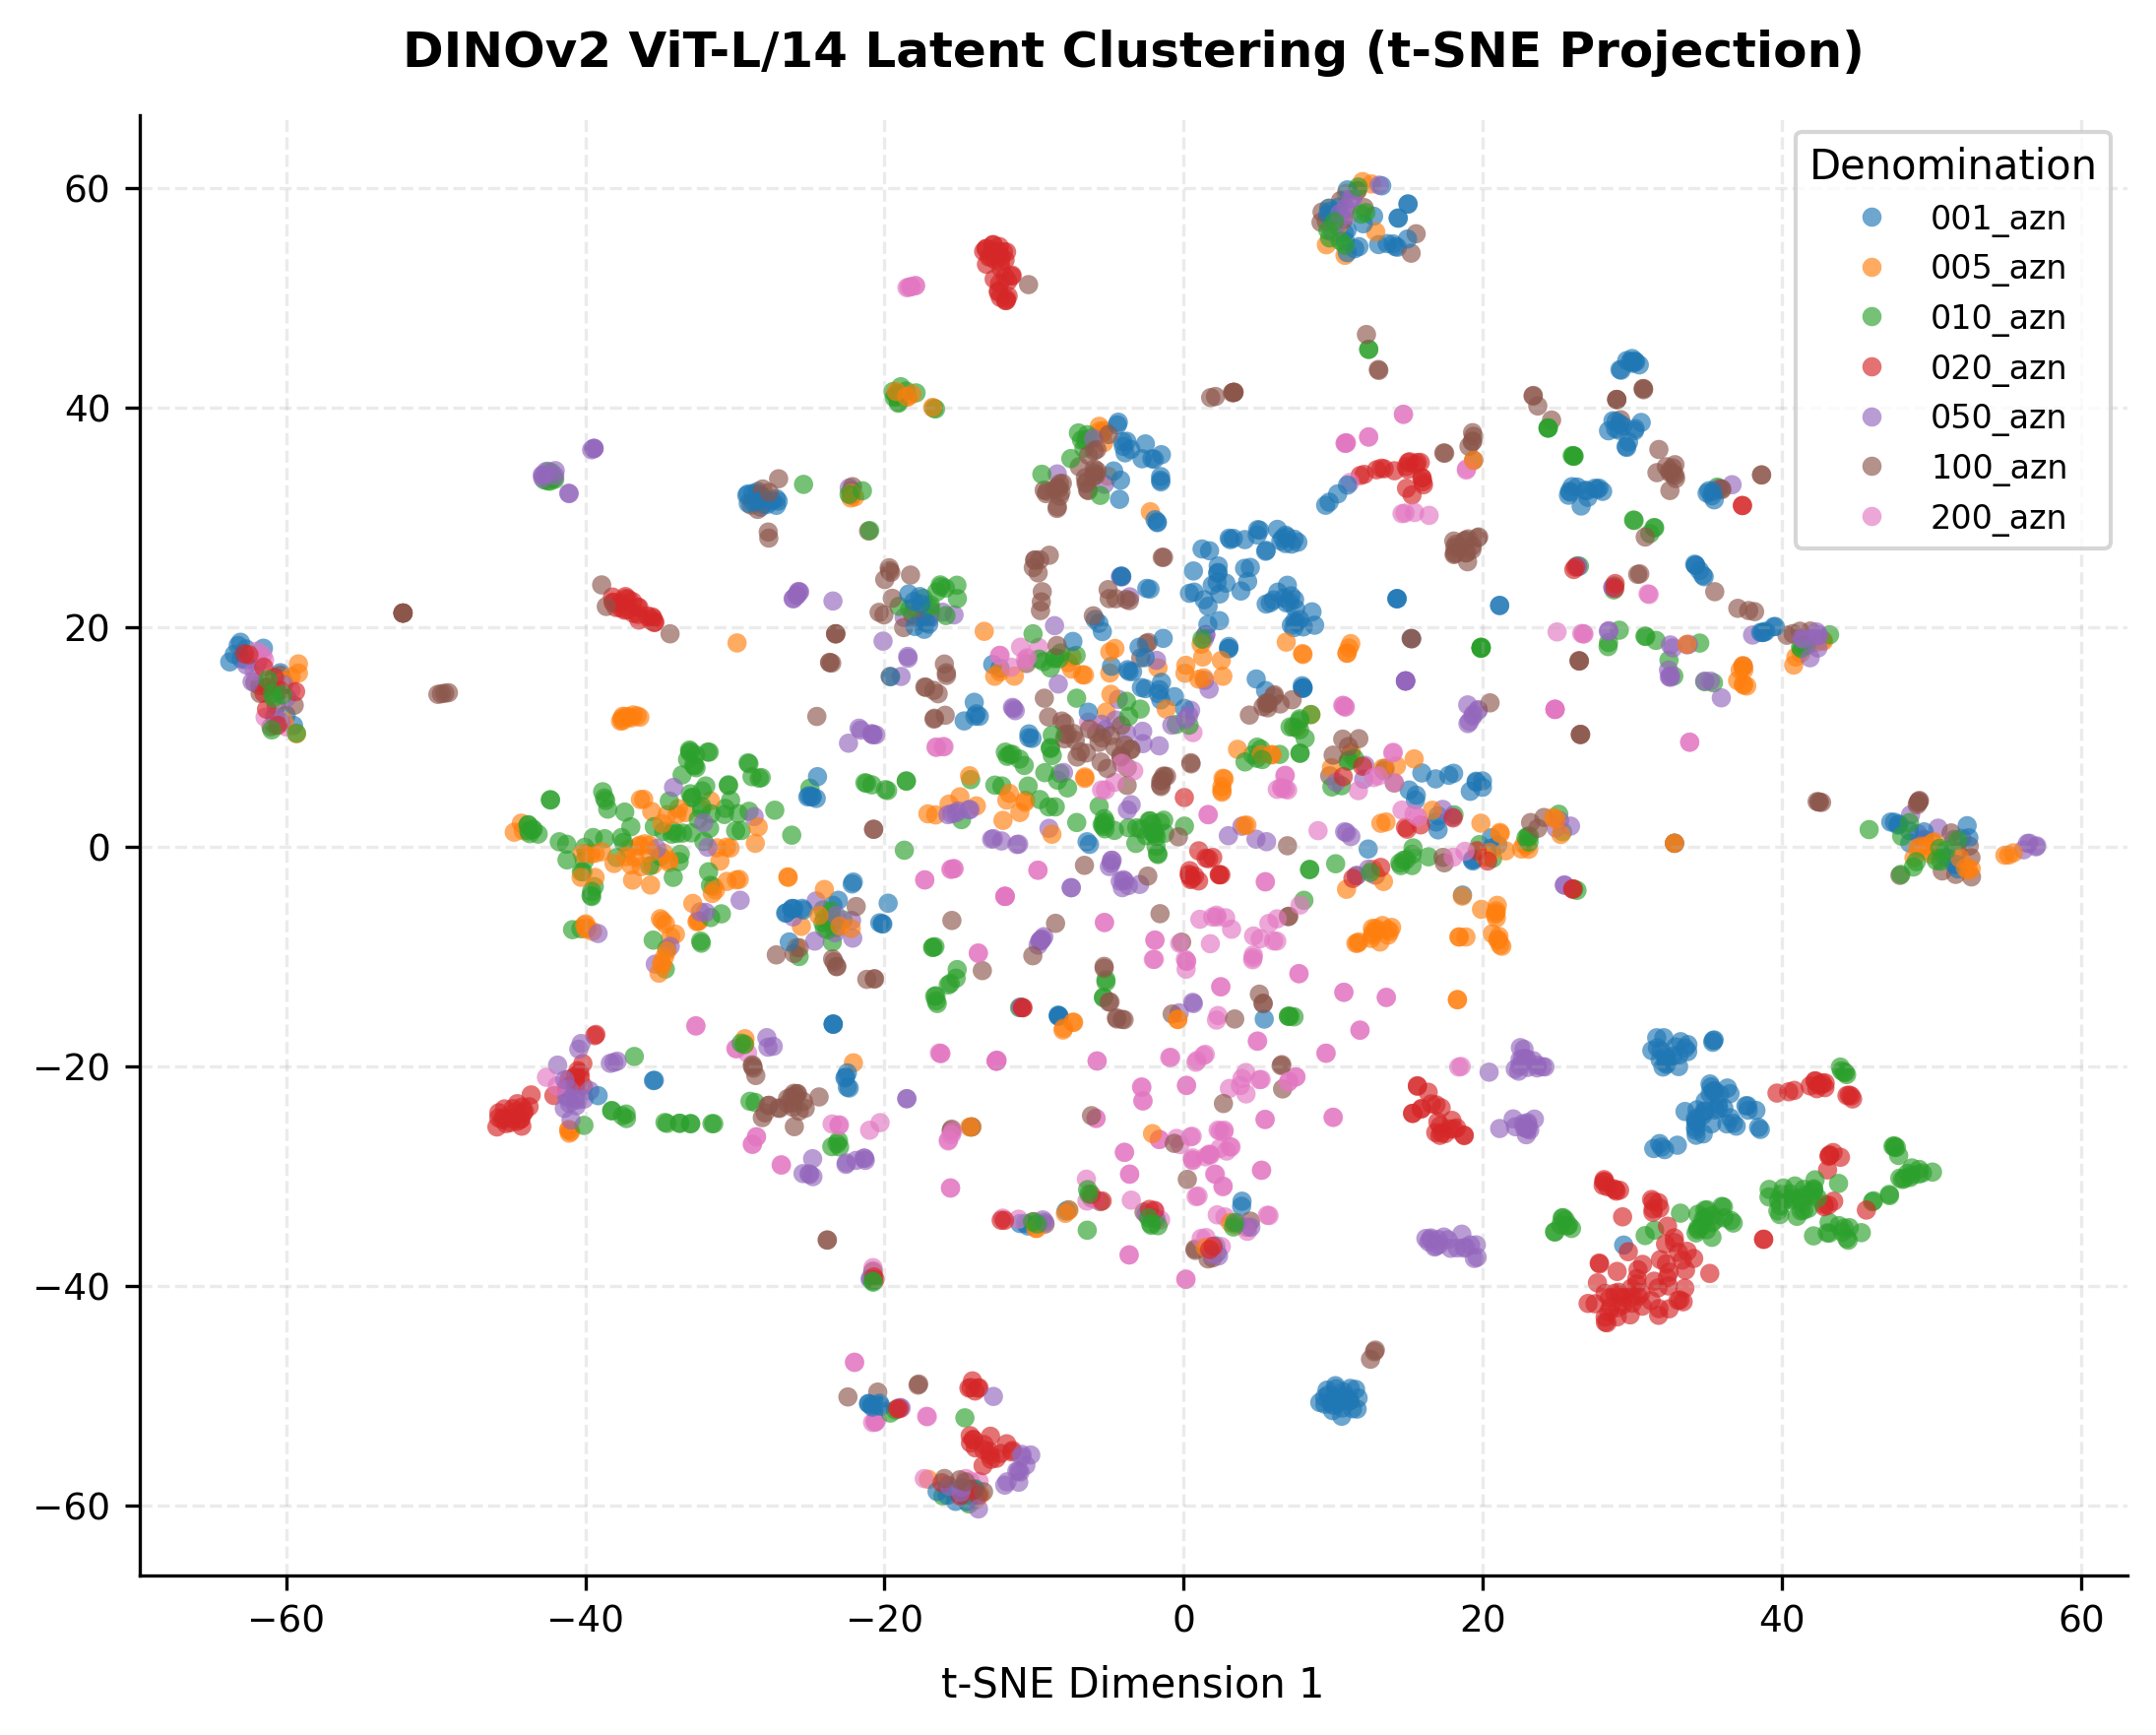
\includegraphics[width=\textwidth,height=0.74\textheight,keepaspectratio]{../reports/figures/embeddings/dinov2_tsne_single.png}
        \end{column}
    \end{columns}
\end{frame}

% ------------------------------------------------------------------------------
% Slide 7 (Page 8): Zero-Leakage Combinatorial Partitioning & Verification
% ------------------------------------------------------------------------------
\begin{frame}{Zero-Leakage Multi-Objective Split Invariant}{Proven 0.00\% Cross-Split Environmental Leakage with Class Balance}
    \begin{columns}[c]
        \begin{column}{0.48\textwidth}
            \centering
            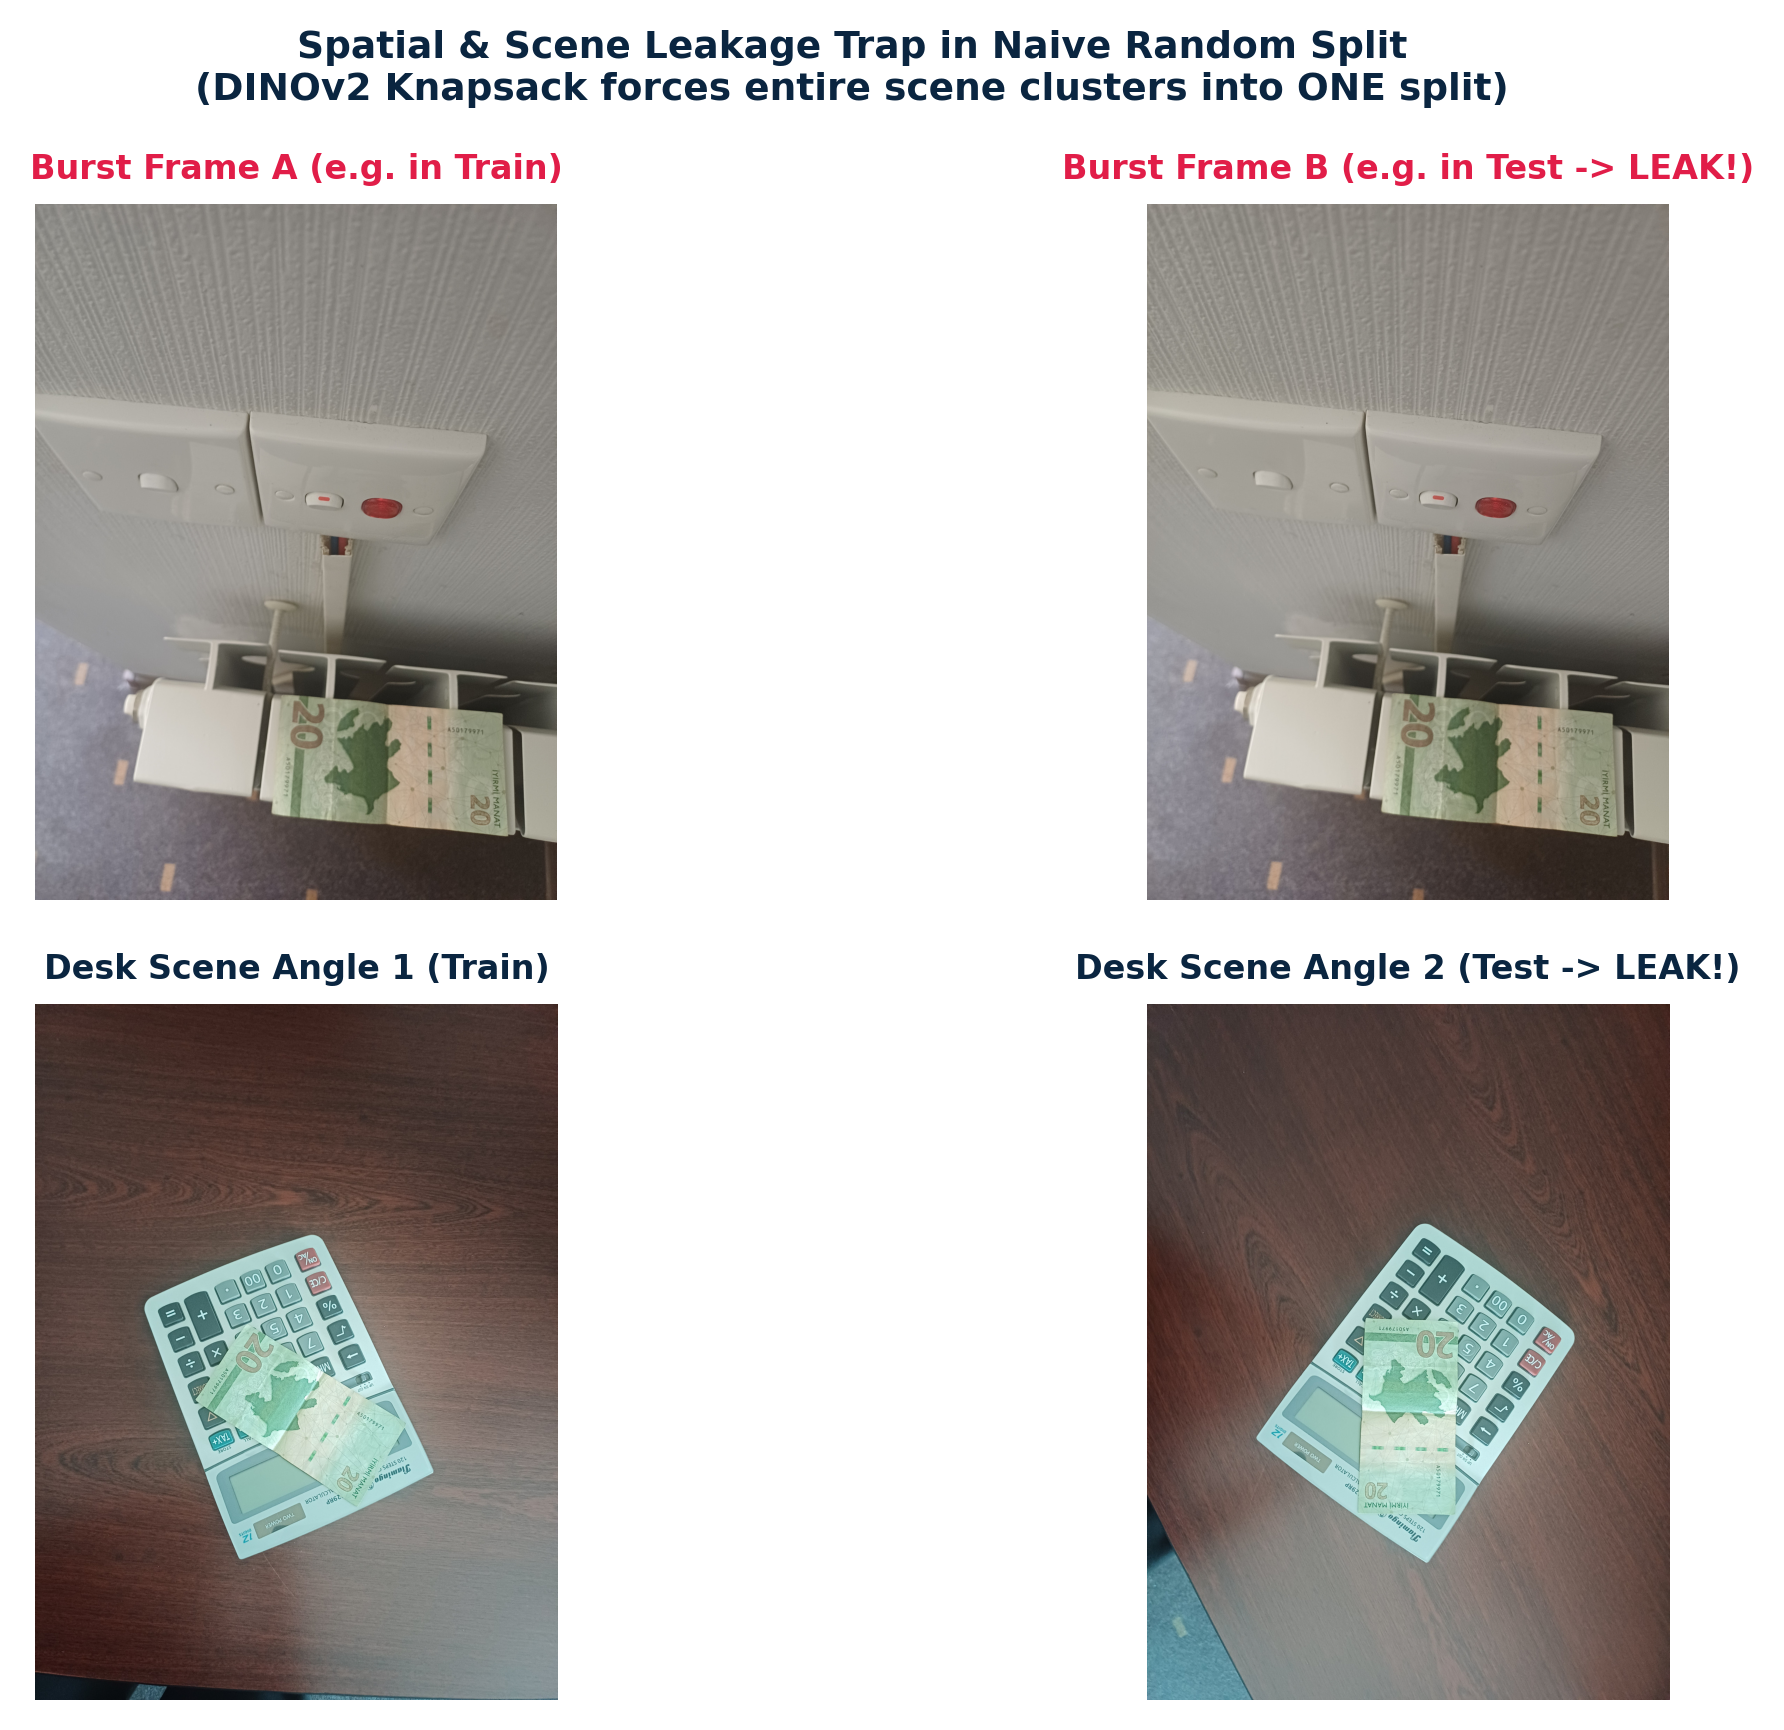
\includegraphics[width=\textwidth,height=0.68\textheight,keepaspectratio]{../reports/figures/splits/zero_leakage_visual_proof.png}
        \end{column}
        
        \begin{column}{0.50\textwidth}
            \begin{techblock}{Combinatorial Routing Pipeline}
                \scriptsize
                \begin{itemize}\setlength{\itemsep}{2pt}
                    \item \textbf{Atomic Knapsack:} Entire meta-scenes routed together.
                    \item \textbf{Minimax Optimization:} Jointly optimizes 70:15:15 split ratio and uniform denomination distribution.
                    \item \textbf{Leakage Guarantee:} Zero burst-pair or desk overlap.
                \end{itemize}
            \end{techblock}
            
            \vspace{0.1cm}
            \begin{card}{Zero-Leakage Verification Audit}
                \tiny
                \begin{itemize}\setlength{\itemsep}{2pt}
                    \item \textbf{Train Split:} 1,760 notes (69.8\%) $\cdot$ 1,774 bounding boxes.
                    \item \textbf{Val Split:} 379 notes (15.0\%) $\cdot$ 401 bounding boxes.
                    \item \textbf{Test Split:} 383 notes (15.2\%) $\cdot$ 386 bounding boxes.
                    \item \textbf{Cross-Split Environmental Leakage:} \textbf{0.00\%} (Proven disjoint).
                \end{itemize}
            \end{card}
            
            \vspace{0.08cm}
            \kpitech{0.00\% Environmental Leakage}{100\% Unseen Test Environments}{Models evaluated on strictly unencountered backgrounds}
        \end{column}
    \end{columns}
\end{frame}
